Mask R-CNN is a framework for instance segmentation. Instance segmentation differs from image classification and semantic segmentation.

Classification, detection and semantic segmentation are image processing tasks  that have been developed in recent years \cite{He.op.2017}\cite{Sharma.21.08.2019}\cite{.08.05.2022}:


\begin{itemize}
    \item \textit{Classification}  is defined as the categorizing of an image to a certain category.
    
    \item \textit{Object Detection} refers to locating and classifying multiple objects within an image. The location is displayed by a squared bounding box.
    
    \item \textit{Semantic Segmentation} is a process where each pixel of an image is classified towards a certain category. This results in a pixel-based mask for each category.
    
\end{itemize}

Although image classification is able to determine the existence of an object within an image, it cannot locate it. Object Detection Models are not only able to detect multiple objects at once, but can also locate them. Nevertheless, Object Detection Models cannot determine the shape of an object. Therefore, Semantic Segmentation was introduced, classifying each pixel and hence defining the shape for each category. However, Semantic Segmentation treats all pixels of a category as one object and cannot distinguish between different instances. Instance Segmentation provides this ability to discern multiple instances of a category.

\section{ (Fast/er) R-CNN}
Mask R-CNN ability for Instance Segmentation  is the end result of the development through three different networks:



\begin{itemize}
    \item \textit{R-CNN} \cite{Girshick.11Nov13} uses three modules for Object Detection. First, it uses Selective Search to generate a list of \ac{RoI}. Second, each proposal is processed through a \ac{CNN} for feature extraction. The third and last step is the classification and localization of the \ac{RoI}.
    
    \item \textit{Fast R-CNN} \cite{Girshick.30Apr15} processes the entire image through a \ac{CNN} to generate a feature map. Each \ac{RoI} is rendered from the feature map and transformed into a uniform size using RoI Pooling. The \ac{RoI} is then fed to a \acl{fc} network in order to be classified and localized by a SoftMax layer at the end.
    
    \item \textit{Faster R-CNN} \cite{Ren.04Jun15} switches the selective search algorithm with a Region Proposal Network and thus significantly improves the prediction time. 
    
\end{itemize}

R-CNN \cite{Girshick.11Nov13} provides the basic architecture for classification and localization. Faster R-CNN \cite{Girshick.30Apr15} improves it in multiple ways. It is using the entire image instead of each \ac{RoI} for the \acl{CNN} and thus increases the training speed. Additionally, the proposals are combined to one batch, which increases the speed even further. Furthermore, the \ac{RoI} Pooling puts the proposals into the same size and thus enabling the usage of a \acl{fc} network to increase the accuracy. Faster R-CNN \cite{Ren.04Jun15} improves the quality and speed by implementing a Region Proposal Network. This network enables the framework to render proposals faster.

\section{ Mask  R-CNN} \label{MaskRCNN}

 Mask R-CNN \cite{He.op.2017} extends Faster R-CNN in two ways (see Figure \ref{fig:maskRcnnFramework}). First, it changes RoI Pooling with RoI Align, which uses bi-linear interpolation to calculate the exact input values based on the four nearest points in each bin. This improves the average precision by approximately three points. Second, Mask R-CNN adds an additional branch to predict a segmentation mask. The additional branch consists of a small \acl{fc} network and predicts a mask for each class. It is only a small computational overhead but enables the network to classify each proposal in a pixel-to-pixel manner. 

 \begin{figure}[!htbp]
 \centering
 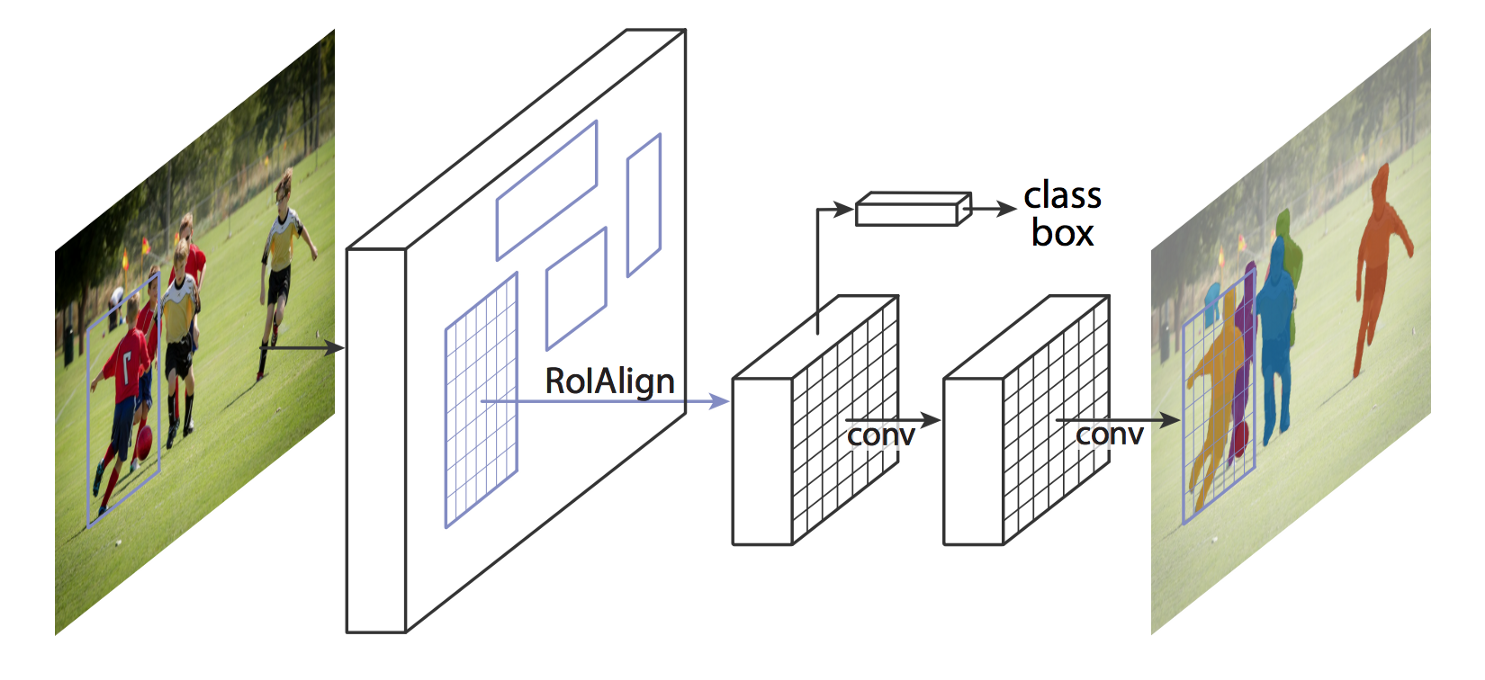
\includegraphics[width=0.5\linewidth]{PICs/maskrcnn.png}
 \caption{Mask R-CNN framework}
 \label{fig:maskRcnnFramework}
 \end{figure}


Like its predecessors, the Mask R-CNN \cite{He.op.2017} framework feeds the entire image to a \ac{CNN} and uses a Region Proposal Network to extract proposals from the feature map. Proposals from one feature map are then put together into one batch. Each proposal is cropped to the same size by RoI Align and then fed to a \acl{fc} network. The proposal is then classified by predicting a discrete probability for each k+1 probability, with the additional class being the background. Mask R-CNN takes a threshold between zero and one as hyper-parameter. If the probabilities fall under the threshold, the proposal is classified as background. Else, the object is localized while simultaneously the segmentation mask is predicted. 

The loss function L is a summation of three different factors:

\begin{equation} \label{lossFunction}   L= L_{cs} + L_{box} + L_{mask} \end{equation}

 \begin{itemize}
    \item \textbf{ \( \label{Lcs}L_{cs}\)} refers to the classification loss determined by the log loss function \( L_{cs}(p,u) = -log(p_{u})\). Mask R-CNN calculates a discrete probability \(p = (p_{0},...,p_{K})\), over K+1 classes, with the additional class being the background and the true class $u$.
    
    \item \textbf{ \( \label{Lbox}L_{box}\)} is defined over tuple $u,v=(v_{x},v_{y},v_{w},v_{h})$ with $v$ being a vector of bounding boxes for each class and the prediction $t=(t^{u}_{x},t^{u}_{y},t^{u}_{w},t^{u}_{h})$ with $u$ being the true class again. If $u$ is the background the $L_{box}$ is 0, otherwise 
    \begin{equation}
        L_{box}(t^{u},v)= \sum_{i \epsilon  \{x,y,w,h\}} smooth_{L_{1}}(t^{u}_{i} - v_{i})
    \end{equation}
    in which
    \begin{equation}
        smooth_{L_{1}}( s= t^{u}_{i} - v_{i})= 
\left\{\begin{matrix}
 0.5s^2 & if|s |<1 \\ |s|-0.5 & otherwise,
\end{matrix}\right.
    \end{equation}
    is a $L_{1}$ loss.
    
    \item \textbf{ \( \label{Lmask}L_{cs}\)} is similar to $L_{box}$ defined as average cross entropy loss. The predicted mask is compared to the ground truth.
\end{itemize}

Although Mask R-CNN predicts bounding boxes and mask for each class, only the losses of the true class from the ground truth contributes to the loss function. This decouples the mask prediction from the classification task. As a result, the mask branch can generate a mask for each class without competition among each other.
Each ROI acts as a sample and all ROI from an image are used as one mini batch. Mask R-CNN then uses Stochastic Gradient Descent \cite{Kiefer.1952}  to optimize the model.
%Barches and stochastic gardient
For details see \citetitle{Girshick.30Apr15} \cite{Girshick.30Apr15} and \citetitle{He.op.2017} \cite{He.op.2017}.